\documentclass[border=4pt]{standalone}
\usepackage{tikz}
\usetikzlibrary{arrows.meta,positioning,calc,fit,backgrounds,patterns,shapes.geometric}
\usepackage{amsmath,amssymb}
\usepackage{mathptmx}
\definecolor{lost}{HTML}{C2362D}
\definecolor{kept}{HTML}{17875A}
\definecolor{evid}{HTML}{3056D3}
\definecolor{ink}{HTML}{1D1D1F}
\definecolor{muted}{HTML}{6E6E73}
\tikzset{
  box/.style={draw=ink!70, rounded corners=2pt, align=center, fill=white, inner sep=4pt, font=\footnotesize},
  arr/.style={-{Stealth[length=2mm]}, draw=ink!70, line width=0.6pt},
  grp/.style={draw=muted!60, dashed, rounded corners=4pt, inner sep=7pt},
  lossbox/.style={draw=lost!80, fill=lost!6, text=lost!85!black, rounded corners=2pt, align=left, font=\footnotesize, inner sep=4pt},
  fixbox/.style={draw=kept!80, fill=kept!7, text=kept!65!black, rounded corners=2pt, align=left, font=\footnotesize, inner sep=4pt},
  dec/.style={diamond, aspect=2.2, draw=ink!70, fill=evid!6, align=center, font=\footnotesize, inner sep=1.5pt},
  lbl/.style={font=\footnotesize\bfseries, text=ink},
}

\begin{document}
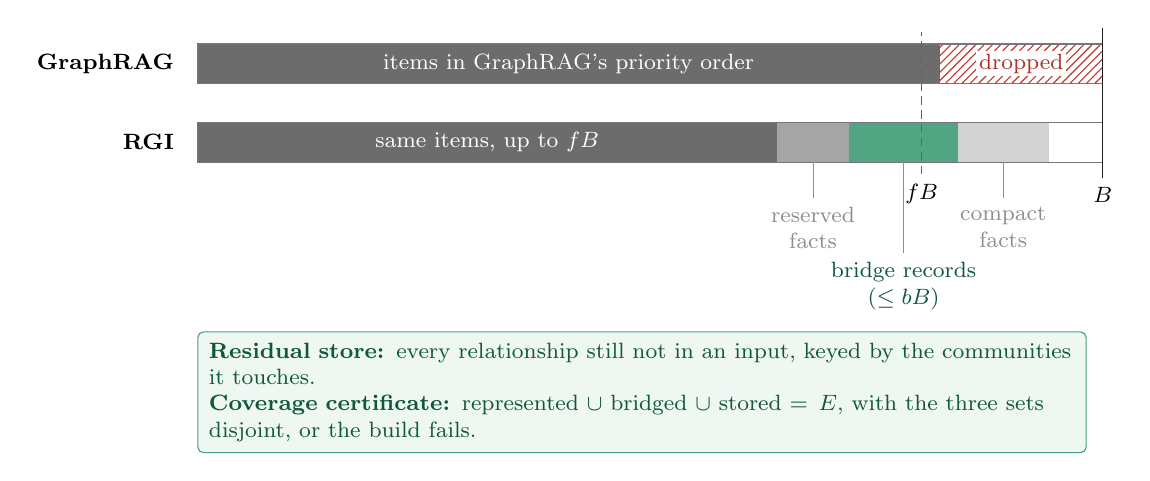
\begin{tikzpicture}[font=\footnotesize, x=1.15cm]
\node[anchor=east, font=\footnotesize\bfseries] at (-0.15,1.45) {GraphRAG};
\fill[ink!65] (0,1.2) rectangle (8.2,1.7);
\fill[pattern=north east lines, pattern color=lost] (8.2,1.2) rectangle (10,1.7);
\draw[ink!60] (0,1.2) rectangle (10,1.7);
\node[text=white] at (4.1,1.45) {items in GraphRAG's priority order};
\node[text=lost!90!black, fill=white, inner sep=1pt] at (9.1,1.45) {dropped};
\node[anchor=east, font=\footnotesize\bfseries] at (-0.15,0.45) {RGI};
\fill[ink!65] (0,0.2) rectangle (6.4,0.7);
\fill[ink!40] (6.4,0.2) rectangle (7.2,0.7);
\fill[kept!75] (7.2,0.2) rectangle (8.4,0.7);
\fill[ink!20] (8.4,0.2) rectangle (9.4,0.7);
\draw[ink!60] (0,0.2) rectangle (10,0.7);
\node[text=white] at (3.2,0.45) {same items, up to $fB$};
\draw[densely dashed, ink!70] (8.0,0.05) -- (8.0,1.85);
\draw[ink] (10,0.0) -- (10,1.9);
\node[anchor=north] at (10,0.0) {$B$};
\node[anchor=north] at (8.0,0.05) {$fB$};
\draw[ink!50] (6.8,0.2) -- (6.8,-0.25) node[anchor=north, align=center] {reserved\\facts};
\draw[ink!50] (7.8,0.2) -- (7.8,-0.95) node[anchor=north, align=center, text=kept!65!black] {bridge records\\($\le bB$)};
\draw[ink!50] (8.9,0.2) -- (8.9,-0.25) node[anchor=north, align=center] {compact\\facts};
\node[fixbox, text width=11cm, anchor=north west] at (0,-1.95) {\textbf{Residual store:} every relationship still not in an input, keyed by the communities it touches.\\ \textbf{Coverage certificate:} represented $\cup$ bridged $\cup$ stored $= E$, with the three sets disjoint, or the build fails.};
\end{tikzpicture}
\end{document}
